\documentclass{beamer}
\usepackage{etoolbox}\newtoggle{printable}\togglefalse{printable}
\usetheme{default}
\usecolortheme{beaver}
\usepackage{listings}
\usepackage{algpseudocode}
\pdfmapfile{+sansmathaccent.map}
\graphicspath{ {Images/} }

\title{Comp310 Demake Proposal}
\author{Alastair Rayner}
\date{\today}

\begin{document}

\maketitle


\begin{frame}{About the DeMake}
	  For this demake project i will be creating Overcooked for the NES. \pause
	  
	  The game will be called Undercooked.\pause
	  
	 This presentation will cover the Concept, Mechanics and Technical Feasibility of the game.
\end{frame}

\begin{frame}{About Overcooked}
    \textbf{Overcooked Examples}
    \center{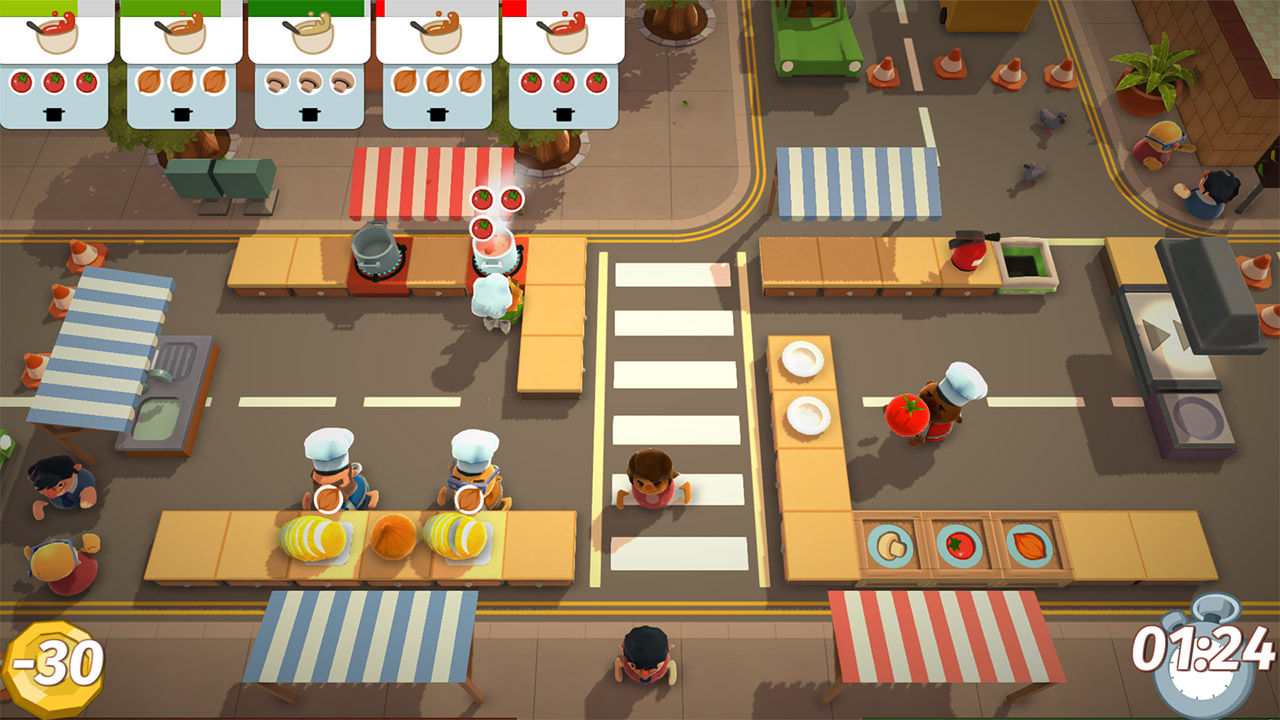
\includegraphics[width=10cm]{Overcooked1}}
    \textit{Image From:} www.psnation.com
\end{frame}

\begin{frame}{About Overcooked}
    \textbf{Overcooked Examples}
    \center{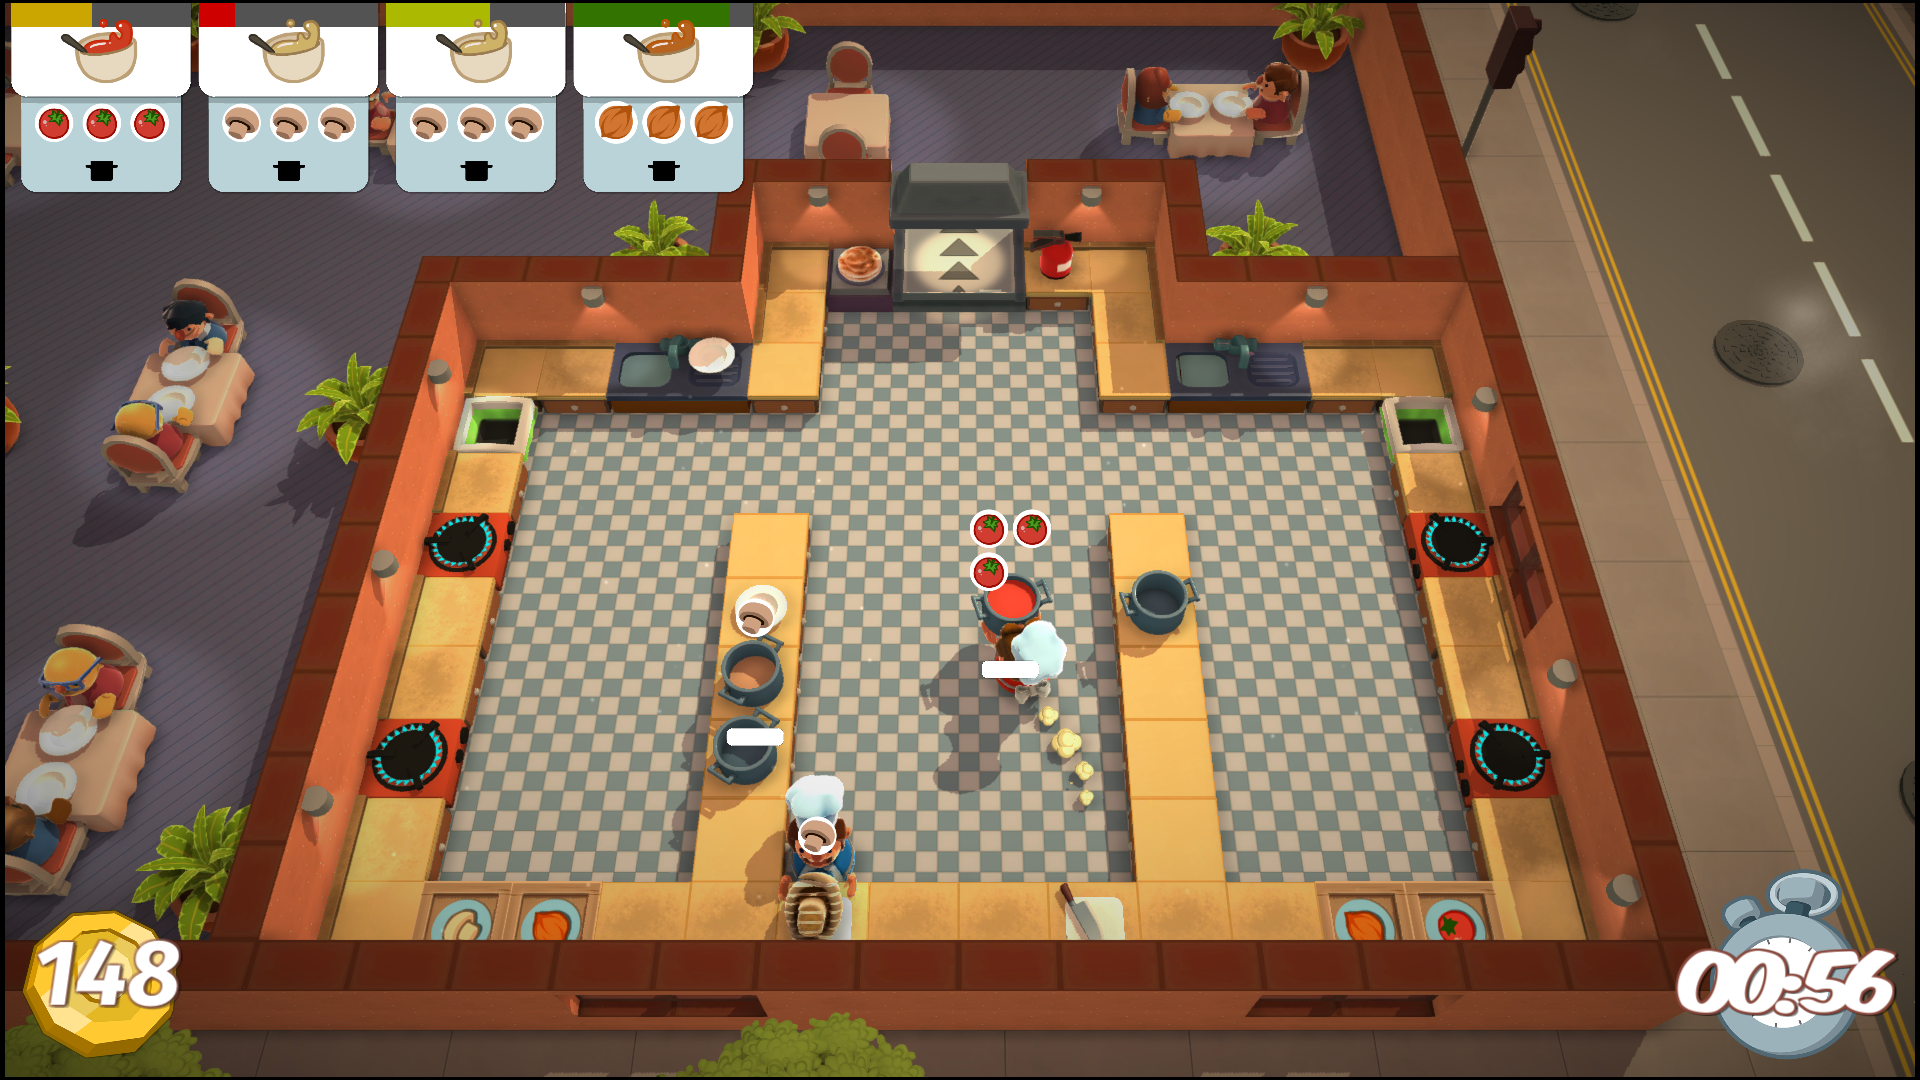
\includegraphics[width=10cm]{Overcooked2}}
    \textit{Image From:} images.nintendolife.com
\end{frame}

\begin{frame}{About Overcooked}
    \textbf{Overcooked Examples}
    \center{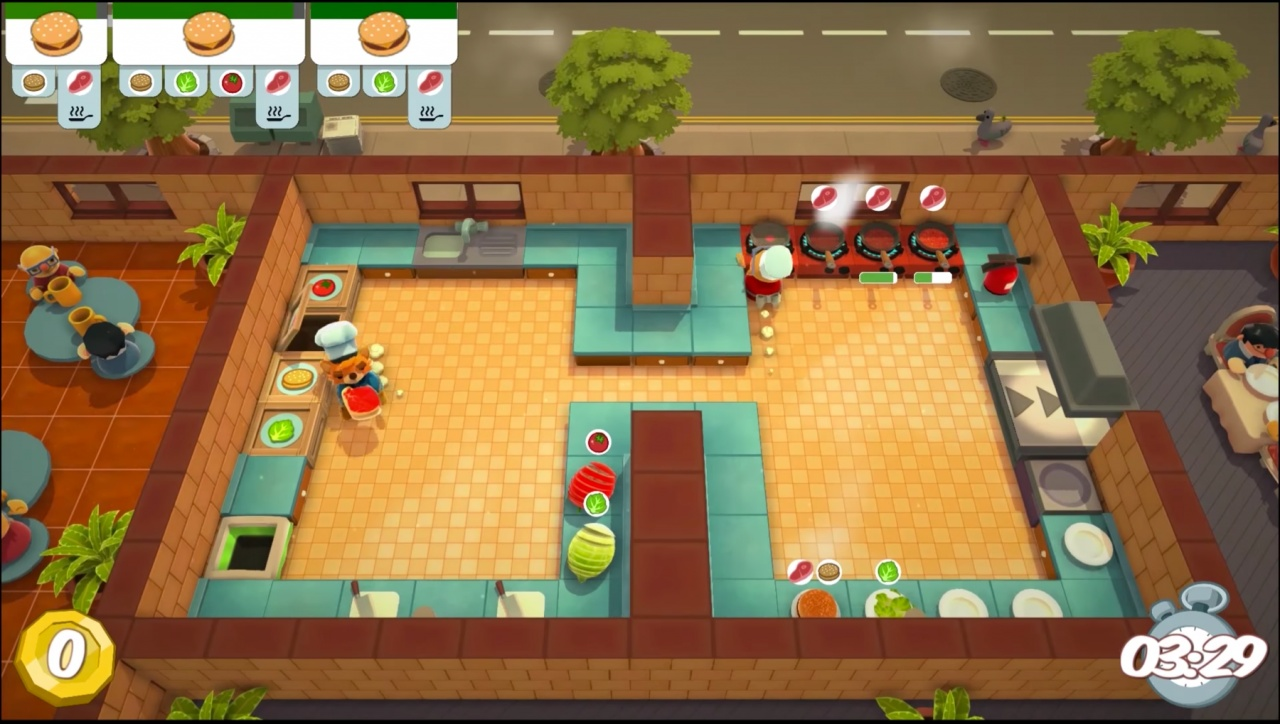
\includegraphics[width=10cm]{Overcooked3}}
   \textit{Image From:} images.nintendolife.com
\end{frame}

\begin{frame}{Concept}		
	\textbf{Game Concept} \pause
		\begin{itemize}
			\item The concept of my demake is a 2D top down cooking game, where the player has to create food as ordered before the time runs out. \pause
			\item The game can be co-op as well as single player. \pause
			\item The players score will increase with every correctly cooked item served.
			
		\end{itemize}
\end{frame}

\begin{frame}{Key Mechanic}		
	\textbf{Core Mechanics} \pause
		\begin{itemize}
		    \item The core merchanics will be the same as Overcooked \pause
			\item Moving items around a kitchen and doing it as efficiently as possible.  \pause
			\item The stretch goals will be to implement co-op and have different levels. \pause
			\item Also have disasters that happen, such as fire that spawns when food is cooked for too long.
			
		\end{itemize}
\end{frame}

\begin{frame}{Technical Feasibility}		
	\textbf{Technical Feasibility} \pause
	
		\begin{itemize}
			\item It will have a simple grid of cells. \pause
			\item The player will hit either A or B buttons to pick up and drop items.  \pause
			\item The game can have a detailed player sprite, consisting of 4 8x8 pixel sprites, and the tiles will be 8x8 pixels.  \pause
			\item The game will have pre-designed levels that the player can walk around in, and interact with certain usable cells, i.e. cooker, chopping board ect.
			
		\end{itemize}
\end{frame}

\begin{frame}{Technical Feasibility}
\center{
    \textbf{The Legend of Zelda}
    This is  a simple example of how I can create the level.}
    \center{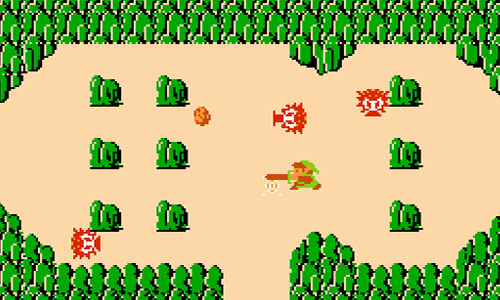
\includegraphics[width=10cm]{Zelda1}}
    \textit{Image From:} www.emuparadise.me
\end{frame}

\begin{frame}{Technical Feasibility}		
 \textbf{Possible Challenges} \pause
		\begin{itemize}
			\item Getting the art to look correct for the food may be a challenge with the limited colour palette. \pause
			\item Knowing what contents are in the burger may be difficult to indicate to the player with few pixels. 	
		\end{itemize}
\end{frame}


\end{document}
